\documentclass[12pt]{article}
\usepackage[a4paper, margin=2cm]{geometry}
\usepackage{amsmath, amssymb}
\usepackage{tikz}
\usepackage{tcolorbox}

% Style basique des zones de réponse
\tcbset{
  case/.style={
    colback=white,
    colframe=black!60,
    boxrule=0.4pt,
    arc=2mm,
    height=3cm
  }
}

\begin{document}

\begin{center}
\Large\textbf{Devoir Surveillé — Vecteurs}\\[0.3cm]
\textit{L’usage de la calculatrice n’est pas autorisé.}
\end{center}

\vspace{0.5cm}
\textbf{Nom :} \dotfill

\vspace{0.5cm}
\hrule
\vspace{0.4cm}

\section*{Automatismes — Calcul littéral, équations, inéquations}

\textbf{1.} Développer, ordonner, réduire :
\[
A = (2x - 1)^2 - (x + 1)^2.
\]
\begin{tcolorbox}[case]\end{tcolorbox}

\textbf{2.} Résoudre dans $\mathbb{R}$ :
\[
3x - \dfrac{1}{3} = x + 5 \qquad \text{et} \qquad 5 - 2(3x - 1) = x + 7
\]
\begin{tcolorbox}[case]\end{tcolorbox}

\textbf{3.} Résoudre dans $\mathbb{R}$ :
\[
2x + 3 < 9 \qquad \text{et} \qquad 5 - x \ge 3x + 1
\]
\begin{tcolorbox}[case]\end{tcolorbox}

\vspace{0.4cm}
\hrule
\vspace{0.4cm}

\section*{Exercice 1 — Construction et démonstration}

\begin{center}
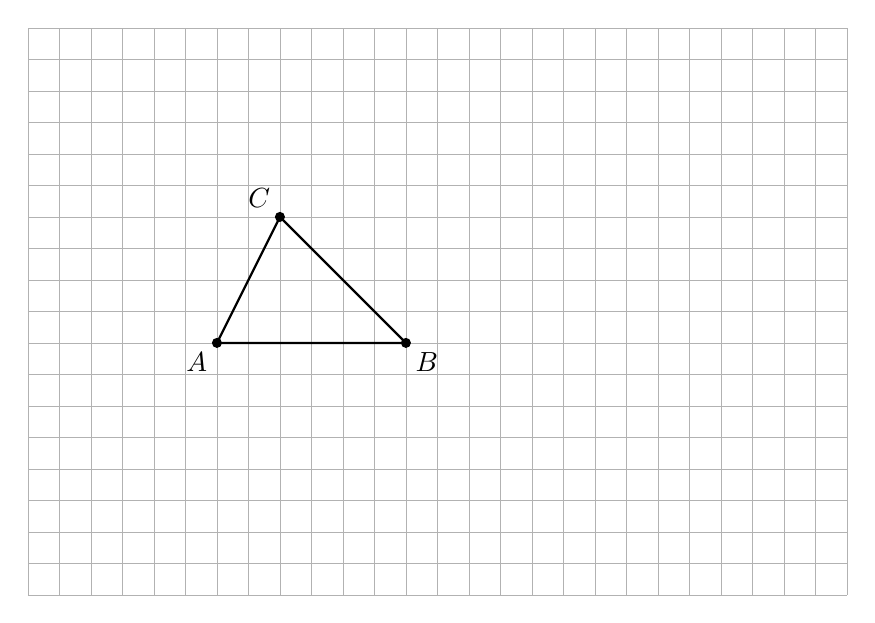
\begin{tikzpicture}[scale=0.8]
  % Grille principale
  \draw[step=0.5cm,gray!60,very thin] (-1,-3) grid (12,6);

  % Points A, B, C visibles (rapprochés)
  \coordinate (A) at (2,1);
  \coordinate (B) at (5,1);
  \coordinate (C) at (3,3);

  % Points et étiquettes
  \filldraw (A) circle (2pt) node[below left] {$A$};
  \filldraw (B) circle (2pt) node[below right] {$B$};
  \filldraw (C) circle (2pt) node[above left] {$C$};

  % Triangle de base
  \draw[thick] (A)--(B)--(C)--cycle;
\end{tikzpicture}

\vspace{0.2cm}
\textit{Utilisez le quadrillage ci-dessus pour construire le triangle $ABC$ et les points demandés.}
\end{center}

\vspace{0.3cm}

On considère un triangle $ABC$.

\textbf{1.} Construire les points $I$, $J$, $K$ et $L$ définis par :
\[
\overrightarrow{AI} = \overrightarrow{AB} + \overrightarrow{AC},\quad
\overrightarrow{AJ} = \overrightarrow{AB} - \overrightarrow{AC},\quad
\overrightarrow{AK} = 2\overrightarrow{AB} - \overrightarrow{AC},\quad
\overrightarrow{BL} = -2\overrightarrow{AC}.
\]

\textbf{2.} En utilisant la relation de Chasles, démontrer que $\overrightarrow{JK} = \overrightarrow{AB}$.
\begin{tcolorbox}[case,height=3.5cm]\end{tcolorbox}

\textbf{3.} Démontrer ensuite que $\overrightarrow{CI} = \overrightarrow{AB}$.
\begin{tcolorbox}[case,height=3.5cm]\end{tcolorbox}


\textbf{4.} En déduire que le quadrilatère $CIKJ$ est un parallélogramme.
\begin{tcolorbox}[case,height=3cm]\end{tcolorbox}

%\textbf{Bonus.} Démontrer que les points $I$, $B$, $J$ et $L$ sont alignés.
%\begin{tcolorbox}[case,height=3.5cm]\end{tcolorbox}



\newpage
\section*{Exercice 2 — Michel Chasles (1793–1880) est votre ami !}

À l’aide de la relation de Chasles, démontrer les égalités suivantes :

\textbf{1.} $\overrightarrow{AB} - \overrightarrow{DC} + \overrightarrow{DA} = \overrightarrow{CB}$
\begin{tcolorbox}[case]\end{tcolorbox}

\textbf{2.} $2\overrightarrow{OA} + \overrightarrow{AC} - \overrightarrow{OC} = \overrightarrow{OA}$
\begin{tcolorbox}[case]\end{tcolorbox}

\textbf{3.} $\overrightarrow{FG} - (\overrightarrow{FA} + \overrightarrow{FB}) - (\overrightarrow{AB} - \overrightarrow{GB}) = \overrightarrow{BF}$
\begin{tcolorbox}[case]\end{tcolorbox}

\textbf{4.} $-\overrightarrow{AB} + \overrightarrow{BC} - \overrightarrow{CA} + 3(\overrightarrow{AB} - \overrightarrow{AC}) - 2\overrightarrow{CB} = \overrightarrow{BC}$
\begin{tcolorbox}[case]\end{tcolorbox}

\vspace{0.4cm}
\textit{Michel Chasles (1793–1880) enseigna à l’École polytechnique dès 1841, puis à la Sorbonne en 1846. Il entra à l’Académie des sciences en 1851 et exposa la relation qui porte son nom dans son \textit{Traité de géométrie supérieure} (1852).}

\end{document}
